\normalfont\normalsize
\chapter{Hardware Platform}

In this chapter we will present the hardware platforms uses in order 

chesti ..... help andrei


\clearpage

\section{The Parrot AR.Drone 2.0}

Parrot AR.Drone is a wifi radio controlled flying quadcopter built by the French company Parrot.
The original drone was released in 2010 and in 2012 it was replaced by version 2.0. Since the launch of the original AR.Drone, more the half a milion units have been sold, making it one of the, if not, the most popular drone on the market.

The reason of its success is not entirely due to the relatively low price of around 300\$ but also because it is very easy to learn how to control the drone and also because of the usb port that accomodate any device using that interface and the linux operating system


\begin{figure}[ht]
\begin{center}
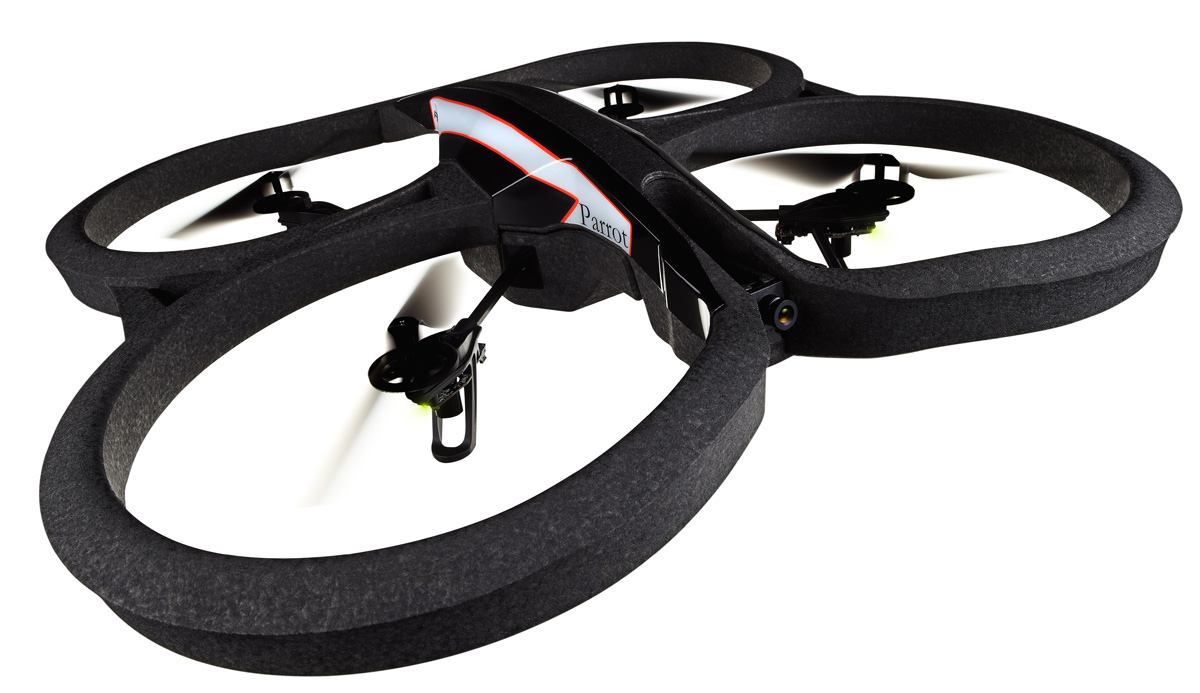
\includegraphics[width=0.9\textwidth]{hw_platform/drone.jpg}
\end{center}
\caption{\small \itshape{The arrot AR.Drone 2.0}}
\end{figure}


Because of those reasons, the Drone has a number of aftermaket modules that can be attached to it like 
the Flight Recorder GPS Module. This module has a built in storage of 4GB for video recording purposes and a built in GPS receiver. This allows the drone to follow a predetermined path of waypoints and to return back from where it took off automatically, all within the limit of the Wi-Fi connection with the control device.
 

The arrot AR.Drone 2.0 specifications are :
\begin{itemize}



\item   1GHz 32 bit ARM Cortex A8 processor with 800MHz video DSP TMS320DMC64x
\item   Linux 2.6.32
\item   1Gbit DDR2 RAM at 200MHz
\item   USB 2.0 high speed for extensions
\item   Wi-Fi b,g,n
\item   3 axis gyroscope 2000°/second precision
\item   3 axis accelerometer +-50mg precision
\item   3 axis magnetometer 6° precision
\item   Pressure sensor +/- 10 Pa precision
\item   Ultrasound sensors for ground altitude measurement
\item   60 fps vertical QVGA camera for ground speed measurement
\item	30 fps 720p front mounted camera 	

\end{itemize}



\clearpage

\section{The Sparrow Dongle}

\begin{figure}[ht]
\begin{center}
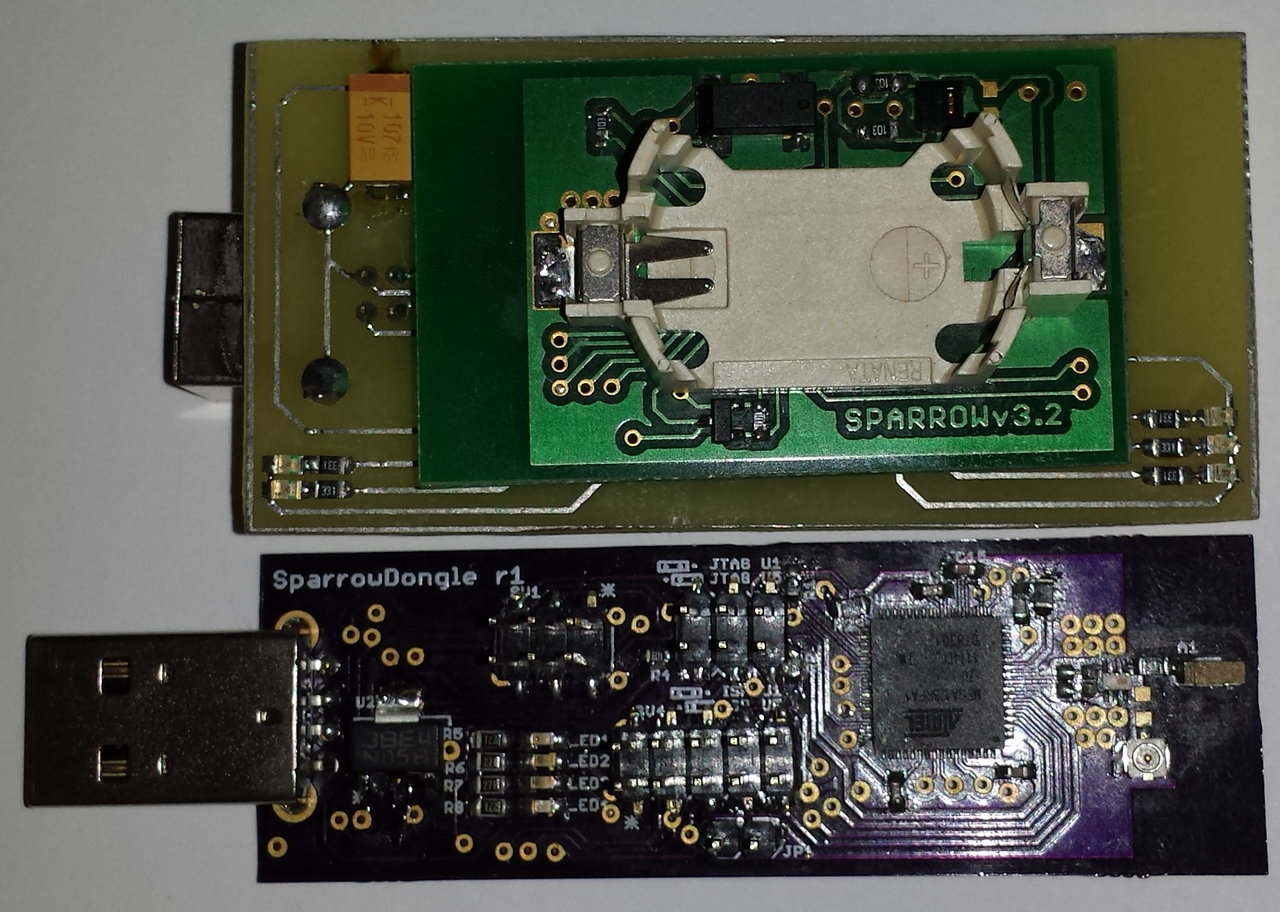
\includegraphics[width=0.9\textwidth]{hw_platform/sparrow.jpg}
\end{center}
\caption{\small \itshape{The Sparrow Dongle next to the SparrowV32}}
\end{figure}

\clearpage

\section{The SparrowV32}

\begin{figure}[ht]
\begin{center}
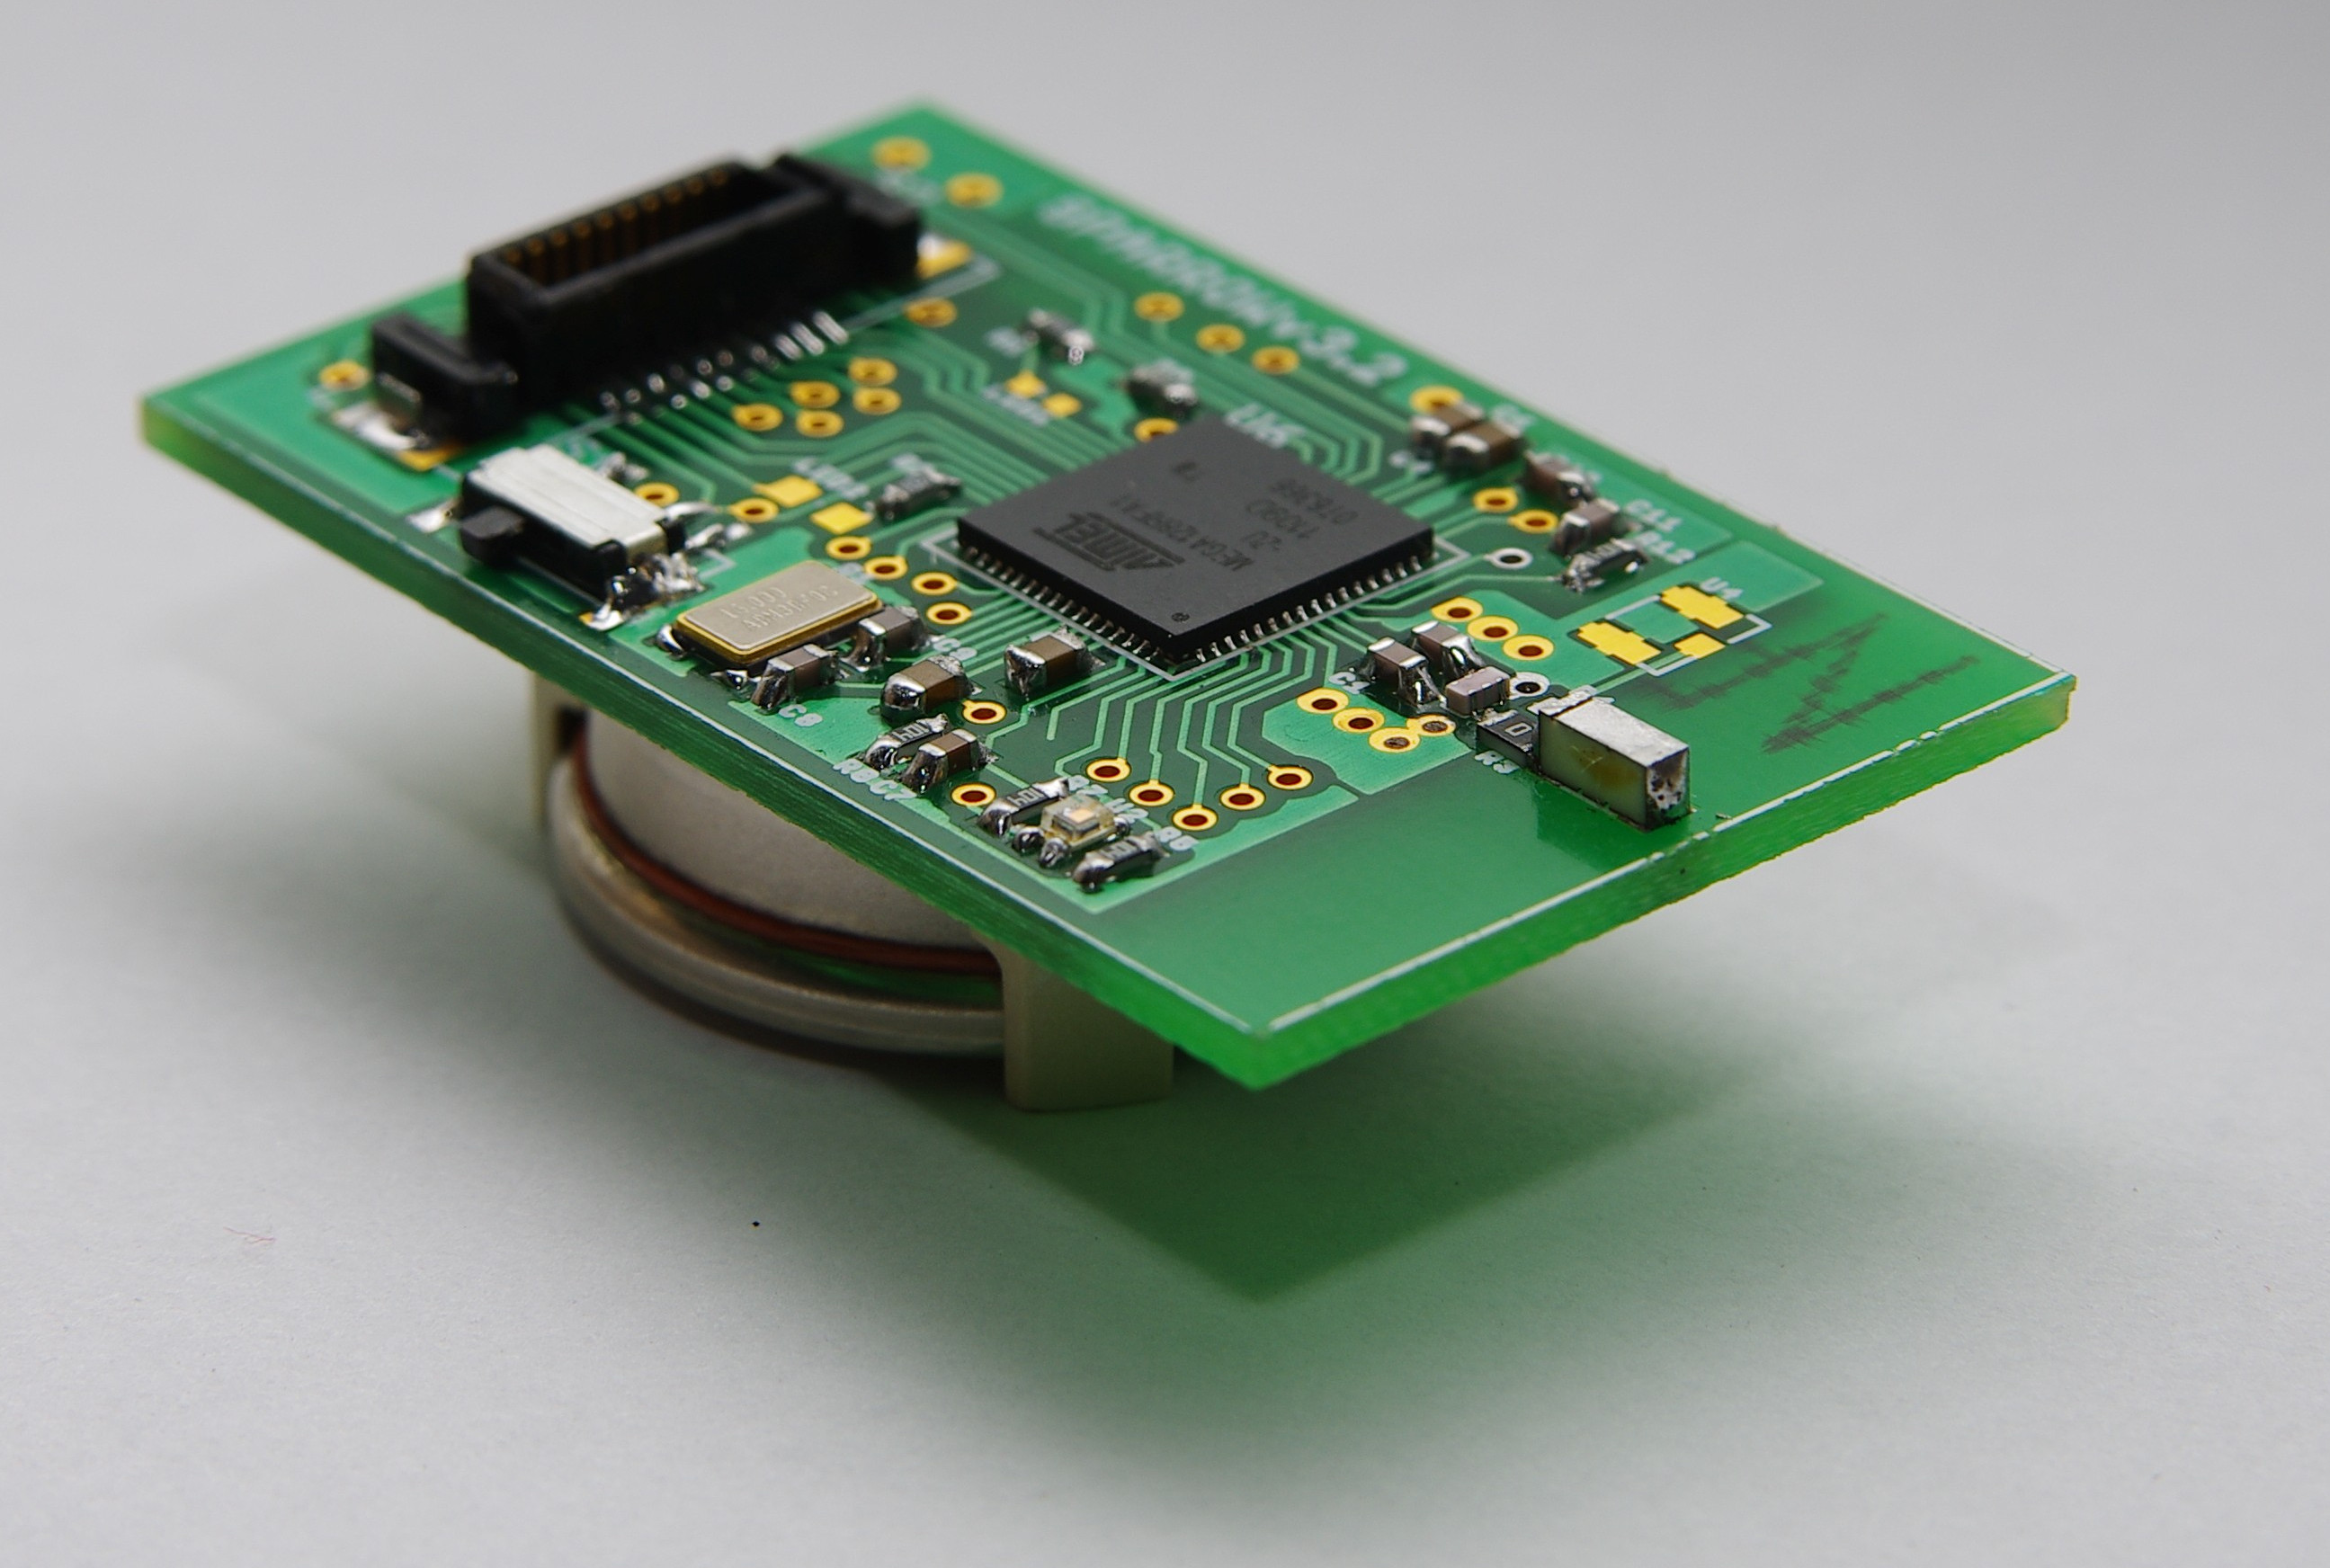
\includegraphics[width=0.9\textwidth]{hw_platform/Sparrowv32.jpg}
\end{center}
\caption{\small \itshape{The SparrowV32}}
\end{figure}
